\documentclass[12pt]{article}

\usepackage{sbc-template}

\usepackage{graphicx,url}

\usepackage{amsmath}

\usepackage{mathtools}

\usepackage[section]{placeins}

\usepackage[brazil]{babel}   

\usepackage[utf8]{inputenc} 

\usepackage{xcolor}

\usepackage{listings}

\usepackage{float}

\newcommand\tab[1][1cm]{\hspace*{#1}}

\definecolor{mGreen}{rgb}{0,0.6,0}
\definecolor{mGray}{rgb}{0.5,0.5,0.5}
\definecolor{mPurple}{rgb}{0.58,0,0.82}
\definecolor{backgroundColour}{rgb}{0.95,0.95,0.92}

\lstdefinestyle{CStyle}{
    backgroundcolor=\color{backgroundColour},   
    commentstyle=\color{mGreen},
    keywordstyle=\color{magenta},
    numberstyle=\tiny\color{mGray},
    stringstyle=\color{mPurple},
    basicstyle=\footnotesize,
    breakatwhitespace=false,         
    breaklines=true,                 
    captionpos=b,                    
    keepspaces=true,                 
    numbers=left,                    
    numbersep=5pt,                  
    showspaces=false,                
    showstringspaces=false,
    showtabs=false,                  
    tabsize=2,
    language=C
}

     
\sloppy

\title{Análise de Paralelismo\\ Fatoração LU}

\author{Paulo Alexandre Piornedo Panucci\inst{1}}


\address{Departamento de Informática -- Universidade Estadual de Maringá
  (UEM)\\
  \email{ra88380@uem.br}
}

\begin{document} 

\maketitle

\begin{abstract}
A sequential code can be written to be parallel executed in a set of threads or process, with the purpose of taking advantage of the core quantity in a machine, or more than one machine, making the program execution faster. It is expected that making a program parallel, it has a significantly better execution time than the sequential program, although there are cases in which the parallelized code has a similar or worst performance compared to the sequential code. In this work will be analyzed the parallel version of LU decomposition algorithm to matrix decomposition. 
\end{abstract}
     
\begin{resumo}
Um código sequencial pode ser escrito para ser executado paralelamente em um conjunto de \textit{threads} ou processos, com finalidade de tirar proveito da quantidade de núcleos presentes em uma máquina, ou de mais de uma máquina, e assim tornar a execução do programa mais rápida. Espera-se que ao paralelizar um determinado programa, ele possua um tempo significantemente melhor que o código sequencial, mas também existem casos em que um código paralelizado tem um desempenho próximo, ou pior, que o sequencial. Neste trabalho será analisada a paralelização do algoritmo Fatoração LU para decomposição de matrizes.  
\end{resumo}


\section{Introdução}\label{sec:intro}

\tab Como observado por \cite{aubanel:1606499}, antes da revolução dos processadores \textit{multicore}, o programador dependia das melhoras de performance apresentadas por processadores conforme o lançamento de novas gerações. Com a estagnação do aumento da taxa de \textit{clock}, poder utilizar múltiplos \textit{cores}  para conseguir rodar um programa tende a tornar a execução mais eficiente dependendo como este problema é modelado.
\\
\tab Hoje conta-se com diretivas de compilação e APIs para paralelizar um código. Um exemplo é o \textit{OpenMP} para a linguagem C/C++. Apesar de existirem alternativas de deixar o trabalho de paralelização para o compilador, aprender a escrever códigos paralelos distribuídos tem suas vantagens. \cite{aubanel:1606499} ainda diz que os compiladores tentam otimizar o código que é dado a eles, porém eles não reescrevem esse código para que ele realmente seja paralelo. Desta forma pode-se dizer que existe uma diferença entre paralelizar um código em C com o OpenMP e escrever um código paralelo utilizando a biblioteca Pthread do C.
\\
\tab As ferramentas citadas acima tem por objetivo auxiliar na escrita de códigos paralelos em memória compartilhada. Para a memória distribuída, pode-se utilizar ferramentas como o MPI (\textit{Message Passing Interface}).

\section{Fundamentação teórica} \label{sec:fund}

\tab Este trabalho abordará a análise de paralelismo do algoritmo da fatoração LU. Desta forma, é importante se conhecer o objetivo desta decomposição, assim como alguns conceitos básicos de paralelismo para se entender esta análise. 

\subsection{fatoração LU}\label{subsec:lu}
\tab A fatoração LU consiste em: dada uma matriz A não singular, existe uma matriz triangular inferior L (\textit{lower}) tal que multiplicada pela matriz triangular superior U (\textit{upper}) o resultado seja A. Logo, esta decomposição pode ser definida pela seguinte fórmula: 
\begin{center}
$A = \text{L} \times \text{U}$.
\end{center}
\tab Uma matriz singular consiste em uma matriz que não admite inversa. Logo a matriz não singular admite a sua inversa.

\subsection{Paralelismo}\label{subsec:paralel}

\tab Serão abordados agora alguns conceitos básicos importantes para se entender o paralelismo a nível de threads e processos e sua análise.

\subsubsection{\textit{Speedup}}\label{subsubsec:speedup}
\tab Ao se escrever um código paralelo a partir de um sequencial, espera-se que seu código paralelo tenha um desempenho de tempo que se aproxima de N vezes melhor que o tempo do código sequencial, sendo este N o número de threads ou processos que serão executadas em paralelo, e este valor é dado pelo \textit{speedup}. 
\\
\tab Quando dividimos o tempo de execução do algoritmo sequencial pelo tempo de execução do algoritmo paralelo, tem-se então o seu \textit{speedup}: 
\begin{center}
$S_p = \frac{T_s}{T_p}$. 
\end{center}
\tab É importante distinguir o tempo decorrido da execução do código, do tempo total levado pela soma dos tempos de execução de cada \textit{thread} ou processo. Para fim de análise de speedup precisa-se do \textit{elapsed time}, que é o tempo decorrido do começo ao fim do programa (ou de uma função paralela específica). 
\\
\tab Quando o \textit{speedup} de um determinado programa paralelo possui um valor maior que o número de \textit{threads} ou processos que executa este código, tem-se então um \textit{speedup} dito superescalar.

\subsubsection{Condição de corrida}\label{subsubsec:racecond}
\tab Ao se escrever um código paralelo, quando \textit{threads} ou processos simultâneas podem competir por algum recurso diz-se que existe condição de corrida neste algoritmo. Pode-se definir como recursos acesso em uma determinada região da memória, e até mesmo o próprio hardware em que o algoritmo está sendo executado. Como um exemplo de disputa de recursos, pode se dar o exemplo que uma determinada \textit{thread} ou processo queira escrever ao mesmo tempo que outra em uma região da memória, ou também a primeira quer ler um resultado que está ao mesmo tempo sendo escrita pela segunda. Como exemplo de disputa de recurso de \textit{hardware}, uma quantidade x de \textit{threads} ou processos que estão prontos para serem executados, porém a máquina contém $\frac{x}{2}$ núcleos de processamento.
\\
\tab Para se resolver problemas de condição de corrida, principalmente de software, deve se usar recursos como \textit{locks} e barreiras ou mensagens síncronas. 
\\
\tab Se existe alguma região crítica em que somente uma \textit{thread} pode estar executando essa região, pode-se utilizar \textit{lock} para não deixar que outras \textit{threads} acessem essa área e \textit{unlock} para liberar para as outras.
\\
\tab Ao se procurar por sincronia em um algoritmo, opta-se pelo uso de barreiras. Quando uma barreira é colocada no algoritmo, isso implica que todas as \textit{threads} devem chegar na mesma região para assim poder dar continuidade na execução.
\\
\tab As mensagens síncronas em programas escritos para memória distribuída acaba fazendo o papel do \textit{lock} e da barreira, apesar de tais estruturas poderem ser utilizadas.
\\
\tab Ter condições de corrida no algoritmo que deseja paralelizar implica em diminuir a possibilidade de ter um \textit{speedup} próximo a quantidade de \textit{threads} ou processos que estão executando. Isto se dá pelo fato de impedir que estes dependam deles mesmos para executar o trabalho que a eles foi dado.

\subsubsection{Balanceamento de carga}\label{subsubsec:cargabalanc}
\tab Independente de como é feita a implementação de um código paralelo, é interessante que os processos ou \textit{threads} tenham um balanceamento execução, ou seja, façam quantidades de trabalho parecidas, para assim alcançar uma melhor performance. 

\subsection{Ferramentas}\label{subsec:cargabalanc}
\tab Serão apresentadas algumas ferramentas utilizadas para  o desenvolvimento do  algoritmo paralelo e sua análise.
\subsubsection{Polybench}
\tab O Polybench é uma coleção de \textit{benchmarks} contendo partes de controle estático, com o propósito de uniformizar a execução e o monitoramento de kernels. 
\\
\tab Desta coleção de \textit{benchmarks} que se teve como base de analise o algoritmo de fatoração LU.  
 
\subsubsection{Pthread}\label{subsubsec:pthread}
\tab Pthread é uma biblioteca para a linguagem C em sistemas \textit{UNIX} que padroniza a programação em \textit{threads} nesse ambiente.
\\
\tab Ao se tratar de uma biblioteca de criação de \textit{threads}, fica a cargo do programador em ditar a maneira como a paralelização funcionará. Desta forma deve-se criar \textit{threads} e passar uma função como argumento para ser executada. Deve-se também fazer a junção dessas \textit{threads}  e se precisar, matá-las.

\subsubsection{Open MPI}\label{subsubsec:ompi}
\tab O Open MPI é uma implementação \textit{open source} de interface de passagem de mensagem, MPI, desenvolvido por um conjunto de acadêmicos, pesquisadores e indústrias.

\section{Proposta}\label{sec:prop}
\subsection{Primeira parte do trabalho}\label{subsec:prop1}
\tab A primeira parte deste trabalho consiste em desenvolver um algoritmo que realize a fatoração LU em uma arquitetura de memória distribuída utilizando a ferramenta Open MPI. Assim, comparar seu desempenho com o desempenho do algoritmo sequencial e  com o algoritmo paralelo para memória compartilhada utilizando a biblioteca Pthread.
\tab A comparação entre estes algoritmos será mostrada através da análise de \textit{speedup} explicada na subseção \ref{subsec:paralel}
\\
\tab O \textit{kernel} do algoritmo sequencial tem a seguinte estrutura: 
\begin{lstlisting}[style=CStyle]
static void kernel_lu(){
  int i, j, k;

  for (k = 0; k < size; k++){
    for (j = k+1; j < size; j++){
      I[k][j] = I[k][j] / I[k][k];
    }
    for(i = k+1; i < size; i++){
      for (j = k + 1; j < size; j++){
        I[i][j] -= I[i][k] * I[k][j];
      }
    }   
  }
}
\end{lstlisting}
\tab O \textit{kernel} do algoritmo Pthread tem a seguinte estrutura: 
\begin{lstlisting}[style=CStyle]
static void *kernel_lu(void *arg){
  int i, j, k;

  int id = *((int *)arg);
  int start = id * cut;
  int end = minimum(start + cut, size);

  for (k = 0; k < size; k++){
    int gap = maximum(k + 1, start);
    for (i = gap; i < end; i++){
      I[i][k] /= I[k][k];
    }
    pthread_barrier_wait(&barrier);
    for(i = gap; i < end; i++){
      for (j = k + 1; j < size; j++){
        I[i][j] -= I[i][k] * I[k][j];
      }
    }
    pthread_barrier_wait(&barrier);
  }

  return NULL;
}
\end{lstlisting}
\tab O \textit{kernel} do algoritmo MPI tem a seguinte estrutura: 
\begin{lstlisting}[style=CStyle]
void ludec_mpi(){

  MPI_Status status;


	MPI_Comm_size(MPI_COMM_WORLD, &world_size);

	MPI_Comm_rank(MPI_COMM_WORLD, &world_rank);

  /*Distribute tasks*/
	if(world_rank == 0){
    populate2Dmatrix(I, size);

		for(int i = 1; i < world_size; i++){
			for(int j = 0; j < size; j++){
        for(int k = 0; k < size; k++){
          MPI_Send(&I[j][k], 1, MPI_DOUBLE, i, 1, MPI_COMM_WORLD);
        }
      }
		}

    // printf("world_rank(%d) distributing the matrix: \n", world_rank);
    // printMatrix(I, size);
	}
  /*Receiving tasks*/
  else{
    for(int i = 0; i < size; i++){
      for(int j = 0; j < size; j++){
        MPI_Recv(&I[i][j], 1, MPI_DOUBLE, 0, 1, MPI_COMM_WORLD, MPI_STATUS_IGNORE);
      }
    }
    // printf("world_rank(%d) receiving the matrix: \n", world_rank);
    // printMatrix(I, size);
	}
  start = MPI_Wtime();
  /*Executing Kernel*/
  for(int k = 0; k < size; k++) {
    MPI_Bcast(I[k], size, MPI_DOUBLE, k % world_size, MPI_COMM_WORLD);
    for(int i = k + 1; i < size; i++) {
      if(i % world_size == world_rank){
        double l = I[i][k] / I[k][k];
        for (int j = k; j < size; j++){
          I[i][j] -= l * I[k][j];
        }
      }
    }
  }
  end = MPI_Wtime();
  /*Distributing Results*/
  int param = (size % world_size - 1 + world_size ) % world_size;
  if(param != 0) {
    if(world_rank == param) {
      for (int i = 0; i < size; i++){
        MPI_Send(I[i], size, MPI_DOUBLE, 0, size + 1, MPI_COMM_WORLD);
      }
    }
    if(world_rank == 0) {
      for(int i = 0; i < size; i++){
        MPI_Recv(I[i], size, MPI_DOUBLE, param, size + 1, MPI_COMM_WORLD, &status);
      }
    }
  }
}
\end{lstlisting}
\subsection{Segunda parte do trabalho}\label{subsec:prop2}
\tab A segunda parte do trabalho consiste em organizar uma arquitetura em \textit{grid} utilizando 13 computadores. a figura \ref{fig:grid} mostra a organização proposta onde os números nos vértices representam os \textit{world ranks} já definidos para exercer cada função. As informações das arestas definem os comunicadores entre cada par de vértice. Cada par de vértice tem seu próprio comunicador.
\\
\tab A maquina com \textit{world rank} 9 será a requisitora. Ela será responsável por requisitar a fatoração LU de matrizes de variadas dimensões. Assim, este computador enviará as matrizes para resolução ao \textit{grid}, sendo o nó de acesso o computador com \textit{world rank} 0. 
\\
\tab Do \textit{world rank} 0 ao 8, os computadores serão responsáveis por fazer o transporte da mensagem até os nós de processamento. A troca de mensagens de um nó ao outro será de forma randômica, com o intuito de analisar os caminhos realizados entre o \textit{grid} até as máquinas processadoras. Como o objetivo é alcançar às máquinas que resolvem o algoritmo, definiu-se que quando um nó nesta malha recebe uma matriz, ele deve mandar para outro nó diferente daquele que enviou os dados pra ele.
\\
\tab Os \textit{world ranks} 10, 11 e 12 são as máquinas que realizam a computação da fatoração LU. Após a computação, esses nós devolvem a matriz fatorada para seus nós adjacentes, e esta matriz fará o caminho mostrado pela figura \ref{fig:return} até o nó requisitor. Após atender todas as requisições, o \textit{world rank} 9 envia uma mensagem, que se espalhará pela malha conforme a figura \ref{fig:kill}, para terminar o algoritmo.
\\
\tab Para análise do comportamento do \textit{grid} será gerado um \textit{log} de uma execução com 4 requisições, com dimensões de 64, 128, 256 e 512. Para exemplificação na subseção \ref{subsec:res2} será mostrado um \textit{log} reduzido de 3 requisições, com dimensões de 64, 128, e 256.
\begin{figure}[ht]
\centering
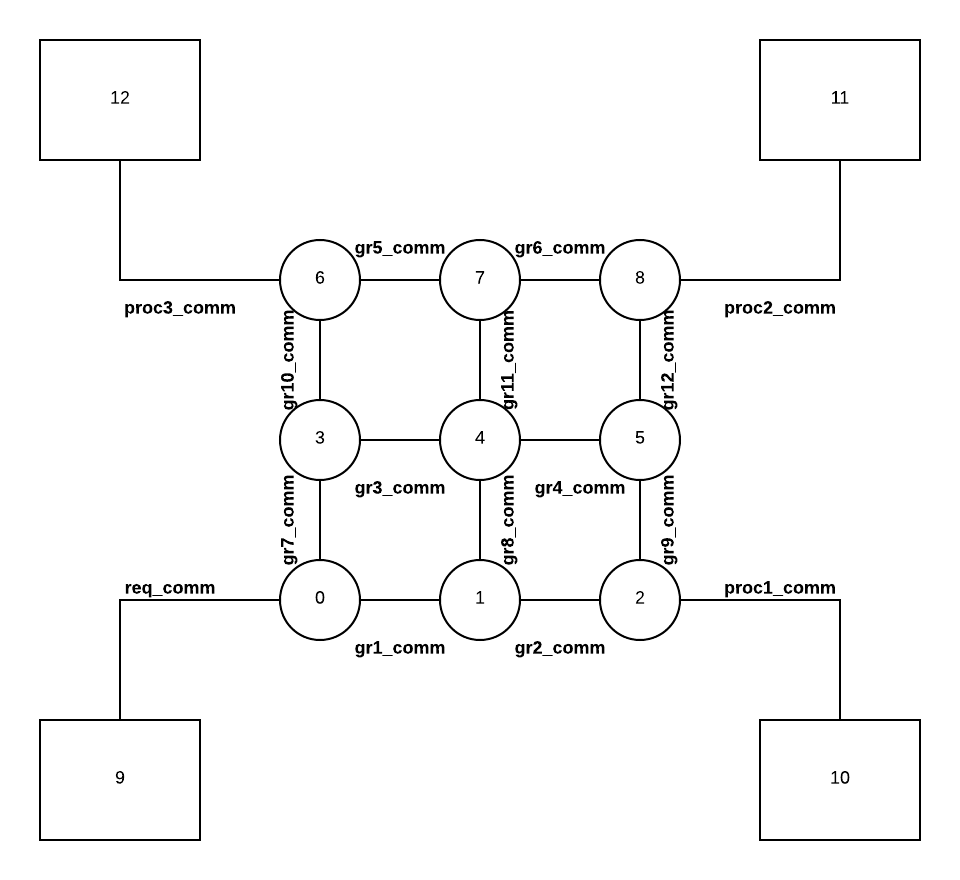
\includegraphics[width=.5\textwidth]{grid-comm.png}
\caption{Formação do \textit{grid}.}
\label{fig:grid}
\end{figure}

\begin{figure}[ht]
\centering
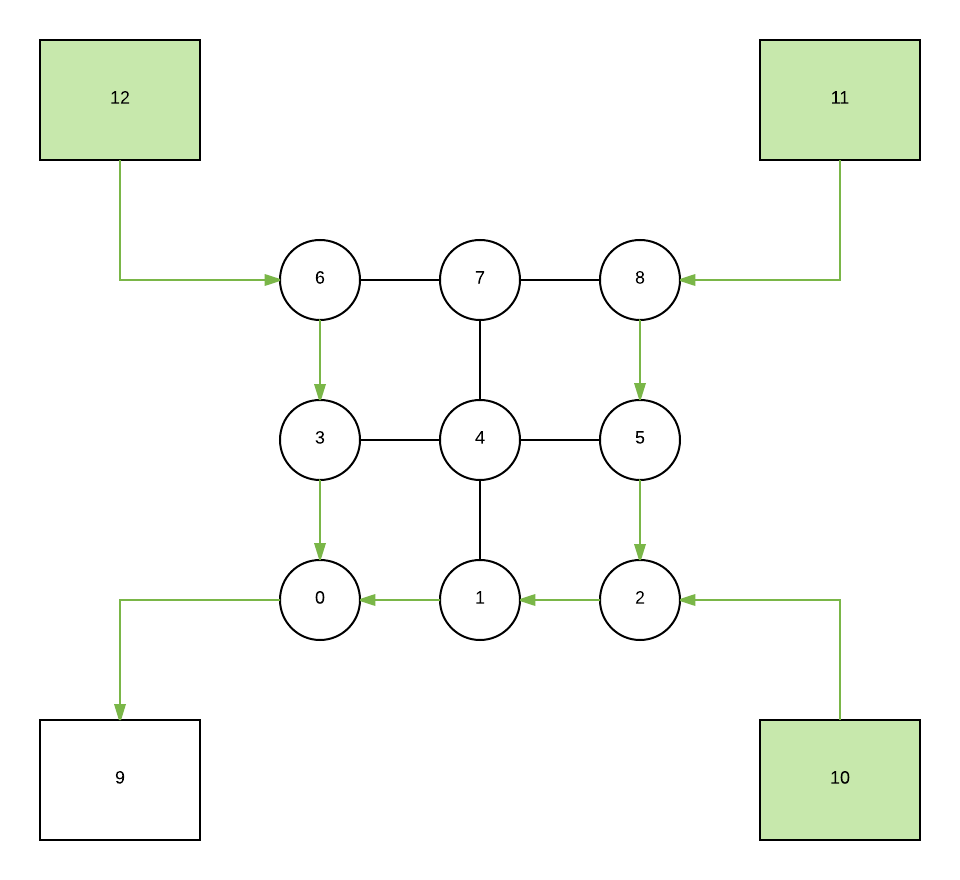
\includegraphics[width=.5\textwidth]{return-grid.png}
\caption{Percurso da mensagem após processamento até o requisitor.}
\label{fig:return}
\end{figure}

\begin{figure}[ht]
\centering
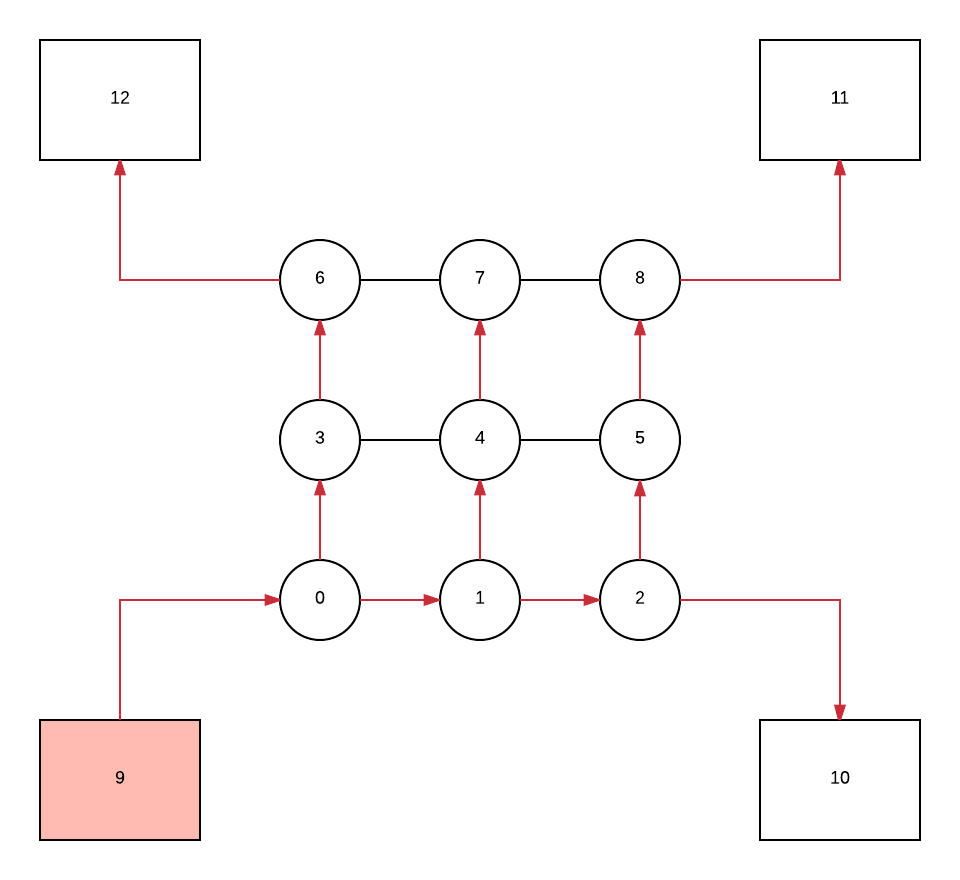
\includegraphics[width=.5\textwidth]{kill-grid.png}
\caption{Percurso da mensagem de finalização do algoritmo.}
\label{fig:kill}
\end{figure}

Quando uma matriz chega a um nó "de borda de processador" (nós 2, 6 e 8), este vértice verifica se o processador está livre. Caso esteja ocupado, a matriz continua andando na malha de forma randômica. Caso contrário, a matriz é mandada para o processador adjacente.

\section{Ambiente experimental}\label{sec:amb}
\tab Foram utilizadas as máquinas presentes no laboratório LIN 02 (Laboratório de Informática 02) do Departamento de Informática da Universidade Estadual de Maringá. Nelas foram rodadas as execuções sequenciais, Pthread e MPI para uma análise justa. 
\\
\tab para cada algoritmo foram realizadas 11 execuções, em que o tempo de execução da primeira é descartado, e entre as outras 10, é retirado o menor e o maior tempo, calculando a média do tempo das execuções restantes.
\\ 
\tab O algoritmo Pthread foi executado para 2, 4, 8 e 16 \textit{threads}. O algoritmo MPI foi executado para 2, 4, 8 e 16 processos. Por problemas de infraestrutura não foi possível executar cada processo do MPI em máquinas diferentes. o LIN 02 só permitia rodar o códio MPI em até 3 máquinas diferentes, impossibilitando a execução para 4 ou mais máquinas. Assim foi utilizado mais processos por máquina, sendo utilizado somente 3 máquinas para todas as execuções.

\section{Resultados}\label{sec:res}
\subsection{Primeira parte do trabalho}\label{subsec:res1}

\tab O gráfico apresentado pela figura \ref{fig:luspeedup} mostra o \textit{speedup} do algoritmo Pthread e MPI. O resultado do Pthread se dá pelo fato de existirem dois pontos de sincronização com barreira dentro laço de repetição principal do \textit{kernel} apresentado na subseção \ref{subsec:prop1}. Para a fatoração ocorrer corretamente, Antes do algoritmo realizar a etapa, chamada de etapa de eliminação, apresentada na linha 16, todas as \textit{threads} devem ter terminado a primeira etapa. Isso acontece pois esta fase escreve resultados em posições utilizadas para o calculo da primeira parte. A ultima barreira na linha 19 sincroniza as \textit{threads} para iniciarem juntas uma nova iteração do laço de repetição principal.
\\
\tab Dada a dimensão de uma matriz para a fatoração LU, existirá um número de sincronização duas vezes maior. Como citado na subseção \ref{subsubsec:racecond}, muita condição de corrida, que necessita de sincronização, atrapalha no desempenho do código sequencial.
\\
\tab Era esperado um melhor resultado de \textit{speedup} do código MPI, pois a necessidade de sincronização constante com barreira é substituída pelas mensagens síncronas. Nota-se um bom \textit{speedup} para dois processos. Isto acontece pois conseguiu-se utilizar dois computadores distintos para executar esses processos. Como explicado na seção \ref{sec:amb} por problemas de infraestrutura só se conseguia executar o algoritmo MPI para até 3 computadores distintos. A interface de passagem de mensagem foi desenvolvida para sanar o problema de troca de mensagens em arquitetura de memória distribuída. Apesar de se conseguir executar para vários processos em uma única máquina, haverá a troca de mensagens entre processos que tem acesso à mesma memória, gerando informações redundantes, assim encarecendo desnecessariamente a execução do algoritmo.

\begin{figure}[H]
\centering
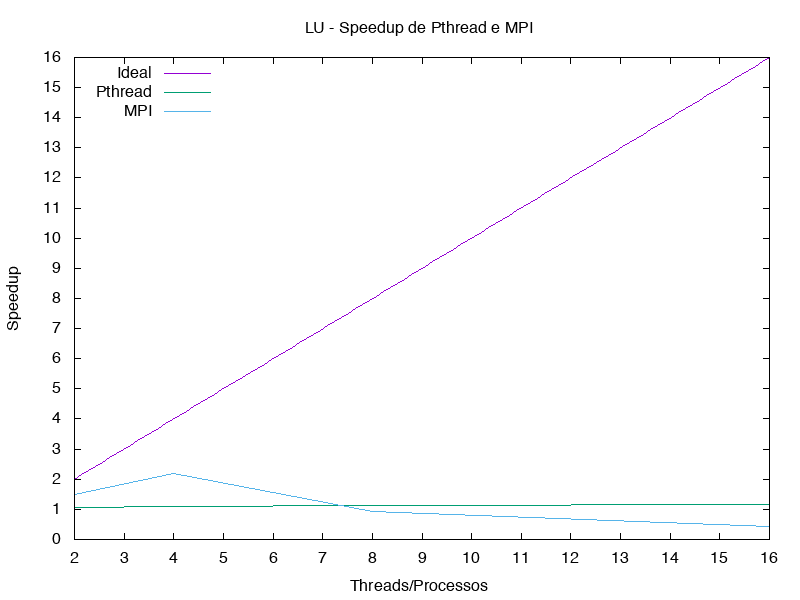
\includegraphics[width=.5\textwidth]{lu-speedup.png}
\caption{\textit{Speedup} do algoritmo Pthread e MPI.}
\label{fig:luspeedup}
\end{figure}

\subsection{Segunda parte do trabalho}\label{subsec:res2}
\subsubsection{\textit{Log} de troca de mensagens no \textit{grid}}
\tab \textbf{Requisitor 9:}
\\
\tab \tab REQUISITOR (WR: 9) - ENVIANDO REQUISIÇÃO [numero de requisição: 1 tamanho 256]
\\
\tab \tab REQUISITOR (WR: 9) - ENVIANDO REQUISIÇÃO [numero de requisição: 2 tamanho 128]
\\
\tab \tab REQUISITOR (WR: 9) - ENVIANDO REQUISIÇÃO [numero de requisição: 3 tamanho 64]
\\
\tab \tab REQUISITOR (WR: 9) - REQUISIÇÃO ATENDIDA [numero de requisição: 1 tamanho 256]
\\
\tab \tab REQUISITOR (WR: 9) - REQUISIÇÃO ATENDIDA [numero de requisição: 3 tamanho 64]
\\
\tab \tab REQUISITOR (WR: 9) - REQUISIÇÃO ATENDIDA [numero de requisição: 2 tamanho 128]
\\
\tab \tab REQUISITOR (WR: 9) - TODAS AS REQUISIÇÕES FORAM ATENDIDAS - ENVIANDO MENSAGEM DE FIM
\\
\tab \tab REQUISITOR (WR: 9) - TODAS AS REQUISIÇÕES FORAM ATENDIDAS - PARANDO AS ATIVIDADES NO REQUISITOR
\\
\\
\tab \textbf{NÓ 0 DO GRID:}
\\
\tab \tab GRID (WR: 0) - RECEBENDO REQUISIÇÃO DE 9 [numero de requisição: 1 tamanho 256]
\\
\tab \tab GRID (WR: 0) - RETRANSMITINDO REQUISIÇÃO PARA 3 [numero de requisição: 1 tamanho 256]
\\
\tab \tab GRID (WR: 0) - RECEBENDO REQUISIÇÃO DE 9 [numero de requisição: 2 tamanho 128]
\\
\tab \tab GRID (WR: 0) - RETRANSMITINDO REQUISIÇÃO PARA 3 [numero de requisição: 2 tamanho 128]
\\
\tab \tab GRID (WR: 0) - RECEBENDO REQUISIÇÃO DE 9 [numero de requisição: 3 tamanho 64]
\\
\tab \tab GRID (WR: 0) - RETRANSMITINDO REQUISIÇÃO PARA 1 [numero de requisição: 3 tamanho 64]
\\
\tab \tab GRID (WR: 0) - RETORNANDO REQUISIÇÃO ATENDIDA [numero de requisição: 1 tamanho 256]
\\
\tab \tab GRID (WR: 0) - RETORNANDO REQUISIÇÃO ATENDIDA [numero de requisição: 3 tamanho 64]
\\
\tab \tab GRID (WR: 0) - RETORNANDO REQUISIÇÃO ATENDIDA [numero de requisição: 2 tamanho 128]
\\
\tab \tab GRID (WR: 0) - PARANDO AS ATIVIDADES NO GRID
\\
\\
\tab \textbf{NÓ 1 DO GRID:}
\\
\tab \tab GRID (WR: 1) - RECEBENDO REQUISIÇÃO DE 0 [numero de requisição: 3 tamanho 64]
\\
\tab \tab GRID (WR: 1) - RETRANSMITINDO REQUISIÇÃO PARA 2 [numero de requisição: 3 tamanho 64]
\\
\tab \tab GRID (WR: 1) - RETORNANDO REQUISIÇÃO ATENDIDA [numero de requisição: 3 tamanho 64]
\\
\tab \tab GRID (WR: 1) - PARANDO AS ATIVIDADES NO GRID
\\
\\
\tab \textbf{NÓ 2 DO GRID:}
\\
\tab \tab GRID (WR: 2) - RECEBENDO REQUISIÇÃO DE 1 [numero de requisição: 3 tamanho 64]
\\
\tab \tab GRID (WR: 2) - PROCESSADOR 10 PRONTO PARA ATENDER A REQUISIÇÃO [numero de requisição: 3 tamanho 64]
\\
\tab \tab GRID (WR: 2) - RETORNANDO REQUISIÇÃO ATENDIDA [numero de requisição: 3 tamanho 64]
\\
\tab \tab GRID (WR: 2) - PARANDO AS ATIVIDADES NO GRID
\\
\\
\tab \textbf{NÓ 3 DO GRID:}
\\
\tab \tab GRID (WR: 3) - RECEBENDO REQUISIÇÃO DE 0 [numero de requisição: 1 tamanho 256]
\\
\tab \tab GRID (WR: 3) - RETRANSMITINDO REQUISIÇÃO PARA 6 [numero de requisição: 1 tamanho 256]
\\
\tab \tab GRID (WR: 3) - RECEBENDO REQUISIÇÃO DE 0 [numero de requisição: 2 tamanho 128]
\\
\tab \tab GRID (WR: 3) - RETRANSMITINDO REQUISIÇÃO PARA 6 [numero de requisição: 2 tamanho 128]
\\
\tab \tab GRID (WR: 3) - RETORNANDO REQUISIÇÃO ATENDIDA [numero de requisição: 1 tamanho 256]
\\
\tab \tab GRID (WR: 3) - RETORNANDO REQUISIÇÃO ATENDIDA [numero de requisição: 2 tamanho 128]
\\
\tab \tab GRID (WR: 3) - PARANDO AS ATIVIDADES NO GRID
\\
\\
\tab \textbf{NÓ 4 DO GRID:}
\\
\tab \tab GRID (WR: 4) - PARANDO AS ATIVIDADES NO GRID
\\
\\
\tab \textbf{NÓ 5 DO GRID:}
\\
\tab \tab GRID (WR: 5) - PARANDO AS ATIVIDADES NO GRID
\\
\\
\tab \textbf{NÓ 6 DO GRID:}
\\
\tab \tab GRID (WR: 6) - RECEBENDO REQUISIÇÃO DE 3 [numero de requisição: 1 tamanho 256]
\\
\tab \tab GRID (WR: 6) - PROCESSADOR 11 PRONTO PARA ATENDER A REQUISIÇÃO [numero de requisição: 1 tamanho 256]
\\
\tab \tab GRID (WR: 6) - RETORNANDO REQUISIÇÃO ATENDIDA [numero de requisição: 1 tamanho 256]
\\
\tab \tab GRID (WR: 6) - RECEBENDO REQUISIÇÃO DE 3 [numero de requisição: 2 tamanho 128]
\\
\tab \tab GRID (WR: 6) - PROCESSADOR 11 PRONTO PARA ATENDER A REQUISIÇÃO [numero de requisição: 2 tamanho 128]
\\
\tab \tab GRID (WR: 6) - RETORNANDO REQUISIÇÃO ATENDIDA [numero de requisição: 2 tamanho 128]
\\
\tab \tab GRID (WR: 6) - PARANDO AS ATIVIDADES NO GRID
\\
\\
\tab \textbf{NÓ 7 DO GRID:}
\\
\tab \tab GRID (WR: 7) - PARANDO AS ATIVIDADES NO GRID
\\
\\
\tab \textbf{NÓ 8 DO GRID:}
\\
\tab \tab GRID (WR: 8) - PARANDO AS ATIVIDADES NO GRID
\\
\\
\tab \textbf{PROCESSADOR 10:}
\\
\tab \tab PROCESSADOR (WR: 10) - PROCESSANDO REQUISIÇÃO [numero de requisição: 3 tamanho 64]
\\
\tab \tab PROCESSADOR (WR: 10) - TODAS AS REQUISIÇÕES FORAM PROCESSADAS - PARANDO AS ATIVIDADES NO PROCESSADOR
\\
\\
\tab \textbf{PROCESSADOR 11:}
\\
\tab \tab PROCESSADOR (WR: 11) - TODAS AS REQUISIÇÕES FORAM PROCESSADAS - PARANDO AS ATIVIDADES NO PROCESSADOR
\\
\\
\tab \textbf{PROCESSADOR 12:}
\\
\tab \tab PROCESSADOR (WR: 12) - PROCESSANDO REQUISIÇÃO [numero de requisição: 1 tamanho 256]
\\
\tab \tab PROCESSADOR (WR: 12) - PROCESSANDO REQUISIÇÃO [numero de requisição: 2 tamanho 128]
\\
\tab \tab PROCESSADOR (WR: 12) - TODAS AS REQUISIÇÕES FORAM PROCESSADAS - PARANDO AS ATIVIDADES NO PROCESSADOR
\\
\\
\section{Conclusão}\label{sec:conc}

\tab A análise feita neste trabalho mostra um desempenho abaixo do esperado para o algoritmo de fatoração LU utilizando a biblioteca Pthread para memória compartilhada. Esperava-se um bom desempenho de \textit{speedup} para o algoritmo MPI, mas foi concluído que esta biblioteca foi desenvolvida para ter um melhor desempenho quando se tem um processo em cada máquina que faz parte da execução. Assim, é interessante o uso de várias máquinas e um algoritmo para memória distribuída para a execução desta fatoração, sendo um fator limitante para isso o custo de se ter várias máquinas independentes para este cálculo.
\\
\tab O \textit{grid} modelado para a segunda parte deste trabalho teve o comportamento esperado de acordo com a proposta da subseção \ref{subsec:prop2}, provado pelo \textit{log} apresentado na subseção \ref{subsec:res2}.
\bibliographystyle{sbc}
\bibliography{sbc-template}
\end{document}
